\documentclass[11pt,a4paper]{article}
\usepackage[margin=2.2cm]{geometry}
\usepackage[utf8]{inputenc}
\usepackage{amsmath,amssymb}
\usepackage{graphicx}
\usepackage{booktabs}
\usepackage{hyperref}
\usepackage{caption}
\usepackage{subcaption}
\graphicspath{{figures/}}

\title{Hands-on Deep Learning: Classification, Regression, and Clustering\\
\large Midterm Exam Report --- Deep Learning (Group 7)}
\author{
  Abdu Fattah Hidayatullah\\{\small NIM 101032300039}
  \and
  Sandy Hidayatullah\\{\small NIM 101032300009}
  \and
  Muhammad Aidil Fadhli Awalludin\\{\small NIM 101032300087}
}
\date{November 2026}

\begin{document}
\maketitle

% Max 18 pages excluding appendices (~5-6 pages per task).
\section{Task 1: Multimodal Classification of Product Defects}
\label{sec:t1}
% Numbers: kode/results/task1/experiment_summary.json & per_class_f1_comparison.csv (python run_all.py --task 1).

We classify 16{,}000 test product units into seven defect classes (\texttt{normal}, \texttt{gores},
\texttt{noda}, \texttt{retak}, \texttt{gelembung}, \texttt{las\_dingin}, and \texttt{kontaminasi})
from 48{,}000 labelled training units. Each unit combines a $64 \times 64$ grayscale surface image
with a $3 \times 128$ press sensor recording (temperature, vibration, current). Evaluation on the
hidden test set uses macro-F1 over all seven classes. Our best model, a three-seed
\textbf{Cross-Attention} multimodal ensemble, achieves \textbf{0.8533} validation macro-F1
($0.8416 \pm 0.0023$ single-seed mean $\pm$ std).

\subsection{Data exploration}
\label{sec:t1-eda}

\paragraph{Class imbalance and metadata.} Nearly half of the 48{,}000 training units are
\texttt{normal} (23{,}888 units, 49.8\%), while the six defect classes range from 11.7\%
(\texttt{gores}, 5{,}623) down to 4.9\% (\texttt{kontaminasi}, 2{,}357); Table~\ref{tab:t1-dist}
lists the full distribution. Units come from 12 press machines, 150 raw-material batches, and three
balanced shifts (\texttt{pagi}, \texttt{siang}, \texttt{malam}).

\paragraph{Missing sensors and train--test domain shift.} In the training set, 2{,}352 units
(4.90\%) have completely missing sensor recordings (all \texttt{NaN}) and 3{,}863 units (8.05\%)
contain at least one \texttt{NaN}; the test set shows almost identical rates (813 units or 5.08\%
completely missing; 1{,}298 or 8.11\% with any \texttt{NaN}). In contrast, the production-line
composition shifts sharply between train and test: training data is dominated by Line~A
(35{,}964 units, 74.9\% vs.\ 12{,}036 or 25.1\% on Line~B), whereas the test set is dominated by
Line~B (9{,}607 units, 60.0\% vs.\ 6{,}393 or 40.0\% on Line~A).

\begin{table}[t]
  \centering
  \caption{Class distribution in the 48{,}000 training units and the 16{,}000 submitted test
  predictions (\texttt{prediksi\_klasifikasi.csv}).}
  \label{tab:t1-dist}
  \small
  \begin{tabular}{lrrrr}
    \toprule
    Class & Train count & Train share & Test pred.\ count & Test pred.\ share \\
    \midrule
    \texttt{normal}      & 23{,}888 & 49.8\% & 9{,}619 & 60.1\% \\
    \texttt{gores}       &  5{,}623 & 11.7\% & 1{,}240 &  7.8\% \\
    \texttt{noda}        &  4{,}773 &  9.9\% & 1{,}332 &  8.3\% \\
    \texttt{las\_dingin} &  4{,}323 &  9.0\% & 1{,}326 &  8.3\% \\
    \texttt{retak}       &  3{,}606 &  7.5\% &   806   &  5.0\% \\
    \texttt{gelembung}   &  3{,}430 &  7.1\% &   960   &  6.0\% \\
    \texttt{kontaminasi} &  2{,}357 &  4.9\% &   717   &  4.5\% \\
    \midrule
    Total                & 48{,}000 & 100.0\% & 16{,}000 & 100.0\% \\
    \bottomrule
  \end{tabular}
\end{table}

\subsection{Preprocessing and architectures}
\label{sec:t1-arch}

\paragraph{Preprocessing.} Training data is split 80/20 with class stratification
(\texttt{random\_state=42}; 38{,}400 train / 9{,}600 validation), and all normalization statistics
are fitted on the training split only. Because raw sensor arrays are stored in \texttt{float16},
valid (non-\texttt{NaN}) readings are cast to \texttt{float64} before computing per-channel means
and standard deviations; computing statistics directly in \texttt{float16} overflows on 4.9M entries
and zeroes out the sensor branch. Missing entries are filled with 0.0 after standardization. During
training we apply random horizontal/vertical flips to images and modality dropout ($p=0.15$, zeroing
the entire sensor tensor) so the model learns to fall back on the image when sensors are absent.

\paragraph{Encoders and fusion strategies.} Both modalities use compact residual
networks~\cite{he2016} producing 128-dimensional representations:
\begin{itemize}
  \item \textbf{Image encoder (2D ResNet):} initial $3\times 3$ convolution (16 channels) followed by
  four strided residual stages (32, 64, 128, 128 channels) reducing $64\times 64$ to $4\times 4$, then
  global average pooling and a linear projection to $\mathbb{R}^{128}$ (or 16 spatial tokens of dim
  128 for attention).
  \item \textbf{Signal encoder (1D ResNet):} initial kernel-5 convolution (16 channels) followed by
  four strided 1D residual stages (32, 64, 128, 128 channels) reducing length 128 to 8, then global
  average pooling and projection to $\mathbb{R}^{128}$ (or 8 temporal tokens for attention).
  \item \textbf{Late fusion:} concatenates the two 128-d embeddings and passes them through a
  two-layer MLP ($256 \to 128 \to 7$) with BatchNorm, ReLU, and dropout $0.3$.
  \item \textbf{Cross-attention fusion:} multi-head attention~\cite{vaswani2017} (4 heads,
  $d=128$) where the 16 image spatial tokens query the 8 signal temporal tokens, followed by residual
  LayerNorm, mean pooling of both streams, concatenation, and an MLP classifier.
\end{itemize}

\subsection{Modality value, label noise, domain shift, and missing sensors}
\label{sec:t1-experiments}

All comparison experiments train for 15 epochs with AdamW ($\text{lr}=10^{-3}$, weight decay
$10^{-4}$), cosine annealing, batch size 128, and seed 42; the final ensemble trains for 18 epochs
across three seeds (42, 123, 999). Before full training, a sanity check overfits one 32-sample batch
for 40 epochs (\texttt{train\_eval.py --sanity-check}), verifying cross-entropy loss $< 0.1$ and
macro-F1 $= 1.00$.

\begin{table}[t]
  \centering
  \caption{Per-class validation F1 and overall macro-F1 (9{,}600 validation units, seed 42).
  Visual defects rely on the image encoder, \texttt{las\_dingin} relies purely on the sensor
  encoder, and multimodal fusion excels on every class.}
  \label{tab:t1-modality}
  \small
  \begin{tabular}{lrrrr}
    \toprule
    Class & Image-Only & Sensor-Only & Late Fusion & Cross-Attention \\
    \midrule
    \texttt{normal}      & 0.827 & 0.704 & 0.899 & \textbf{0.905} \\
    \texttt{gores}       & 0.710 & 0.049 & 0.750 & \textbf{0.755} \\
    \texttt{noda}        & 0.872 & 0.092 & \textbf{0.874} & 0.871 \\
    \texttt{retak}       & 0.521 & 0.673 & 0.718 & \textbf{0.735} \\
    \texttt{gelembung}   & 0.556 & 0.760 & 0.776 & \textbf{0.794} \\
    \texttt{las\_dingin} & 0.000 & \textbf{0.936} & 0.933 & 0.934 \\
    \texttt{kontaminasi} & 0.884 & 0.008 & 0.899 & \textbf{0.899} \\
    \midrule
    \textbf{Macro-F1}    & 0.624 & 0.460 & 0.836 & \textbf{0.842} \\
    \bottomrule
  \end{tabular}
\end{table}

\paragraph{Value of each modality.} Table~\ref{tab:t1-modality} reveals a clean division between
modalities. The \textbf{Image-Only} 2D ResNet (macro-F1 0.624) detects surface defects accurately
(\texttt{kontaminasi} 0.884, \texttt{noda} 0.872, \texttt{gores} 0.710) but is completely blind to
\texttt{las\_dingin} (0.000). Conversely, the \textbf{Sensor-Only} 1D ResNet (macro-F1 0.460)
detects \texttt{las\_dingin} with 0.936 F1 and outperforms images on \texttt{gelembung} (0.760 vs.\
0.556) and \texttt{retak} (0.673 vs.\ 0.521), yet cannot see surface-only defects
(\texttt{kontaminasi} 0.008, \texttt{gores} 0.049, \texttt{noda} 0.092). Combining both modalities
adds over +0.21 macro-F1: \textbf{Late Fusion} reaches 0.8356 and \textbf{Cross-Attention} reaches
\textbf{0.8419}, with the largest cross-attention gains on the subtle dual-modality classes
\texttt{gelembung} (+0.018) and \texttt{retak} (+0.017).

\begin{table}[t]
  \centering
  \caption{Summary of Task 1 robustness, domain-shift, and final 3-seed validation results
  (9{,}600 validation units; from \texttt{kode/results/task1/experiment\_summary.json}).}
  \label{tab:t1-results}
  \small
  \begin{tabular}{lrrr}
    \toprule
    Experiment / Model & Overall F1 & Line A F1 & Line B F1 \\
    \midrule
    Image-Only 2D ResNet                                      & 0.6243 & --     & --     \\
    Sensor-Only 1D ResNet                                     & 0.4601 & --     & --     \\
    Late Fusion (global norm, LS $\epsilon=0.1$)              & 0.8356 & 0.8755 & 0.7004 \\
    Late Fusion (no label smoothing, $\epsilon=0.0$)          & 0.8369 & --     & --     \\
    Late Fusion + Per-Line Norm (image \& sensor)             & 0.8269 & 0.8704 & 0.6807 \\
    Cross-Attention (global norm, LS $\epsilon=0.1$)          & 0.8419 & --     & --     \\
    Cross-Attention + Per-Line Norm (image \& sensor)         & 0.8415 & 0.8797 & 0.7099 \\
    Cross-Attention with 100\% Missing Sensor                 & 0.5777 & --     & --     \\
    Cross-Attention on Natural Missing-Sensor Val Subset      & 0.5497 & --     & --     \\
    \midrule
    Final Cross-Attention (3 seeds: 42, 123, 999)             & $0.8416 \pm 0.0023$ & -- & -- \\
    \textbf{Final 3-Seed Probability Ensemble}                & \textbf{0.8533} & \textbf{0.8886} & \textbf{0.7328} \\
    \bottomrule
  \end{tabular}
\end{table}

\paragraph{Imperfect labels.} Using the trained multimodal model to flag high-confidence
disagreements (predicted probability $\ge 0.85$) identifies \textbf{339 likely mislabels} out of
9{,}600 validation units (3.53\%). Comparing standard cross-entropy ($\epsilon=0.0$, macro-F1
0.8369) against label smoothing~\cite{szegedy2016} ($\epsilon=0.1$, macro-F1 0.8356) yields nearly
identical scores on the noisy validation labels (difference 0.0013), while preventing overconfident
memorization of corrupted inspector labels; we keep $\epsilon=0.1$ for regularization in the final
training recipe.

\paragraph{Domain shift across production lines.} Evaluating by production line exposes a large
domain gap: under global normalization, Late Fusion scores 0.8755 on Line~A but drops to 0.7004 on
Line~B ($-0.175$). Standardizing both images and sensors per line slightly lowers Late Fusion
(0.8269 overall; Line~B 0.6807) because Line~B has $3\times$ fewer training samples for estimating
statistics, whereas \textbf{Cross-Attention + Per-Line Norm} lifts both lines (Line~A 0.8797, Line~B
0.7099; overall 0.8415). Because our automated selection criterion compared Late Fusion per-line
against global normalization before picking the architecture, the final ensemble used
Cross-Attention with global normalization; ensembling three seeds further lifts Line~B to
\textbf{0.7328} (Line~A \textbf{0.8886}).

\paragraph{Missing modality robustness.} Trained with 15\% sensor modality dropout, the chosen
Cross-Attention model retains \textbf{0.5777} macro-F1 even when 100\% of validation sensors are
wiped to \texttt{NaN} (approaching the dedicated Image-Only ceiling of 0.6243), and achieves
\textbf{0.5497} macro-F1 on the naturally missing-sensor validation subset---confirming graceful
fallback to visual features rather than collapsing.

\subsection{Final model and test predictions}
\label{sec:t1-final}

The final model trains \textbf{Multimodal Cross-Attention} for 18 epochs across three random seeds:
seed 42 (0.8428), seed 123 (0.8435), and seed 999 (0.8384), giving a mean validation macro-F1 of
$0.8416 \pm 0.0023$. Averaging the softmax probabilities of the three checkpoints raises validation
macro-F1 to \textbf{0.8533} (Line~A 0.8886, Line~B 0.7328). Applied to the 16{,}000 hidden test
units, \texttt{prediksi\_klasifikasi.csv} predicts all seven classes in proportions consistent with
the training distribution and the Line~A $\to$ Line~B shift (Table~\ref{tab:t1-dist}).

\clearpage
\section{Task 2: Remaining Useful Life Regression}
% Numbers: kode/results/task2/*.json (python run_all.py --task 2). Supporting material: Appendix.

We predict the remaining useful life (RUL) of 300 press machines at their last recorded cycle,
from 900 run-to-failure histories. Each cycle has three operating settings and 21 sensors; the data
structure and the asymmetric score follow the C-MAPSS benchmark~\cite{saxena2008damage}. The best
architecture, a GRU, reaches an RMSE of $19.2 \pm 0.8$ cycles in five-fold cross-validation by
machine, and the submitted predictions average five GRUs. Supporting figures and tables are in
Appendix~\ref{app:t2}.

\subsection{Exploration and preprocessing}
\label{sec:t2-prep}

\paragraph{Operating settings and normalisation.} The settings take six discrete combinations
(Fig.~\ref{fig:t2-regimes}a), which KMeans ($k=6$) separates perfectly. The regime changes in 83\%
of consecutive cycles and explains 37--100\% of each sensor's variance, so raw readings jump between
levels and hide the slow wear trend (Fig.~\ref{fig:t2-regimes}b). We therefore z-score each sensor
within its regime, using statistics from training machines only. Noise levels are almost equal
across regimes (max/min standard deviation $\le 1.024$), so this removes the offset without
distorting the signal: the trend becomes visible (Fig.~\ref{fig:t2-regimes}c) and the rank
correlation of s04 with RUL rises from 0.28 to 0.71 in absolute value.

\begin{figure}[t]
  \centering
  \includegraphics[width=\linewidth]{t2_regimes}
  \caption{(a) The operating settings form six regimes. (b) Raw s04 of one machine, coloured by
  regime. (c) The same sensor after per-regime normalisation shows the wear trend.}
  \label{fig:t2-regimes}
\end{figure}

\paragraph{Sensors, gaps and spikes.} Seven sensors (s01, s05, s06, s10, s16, s18, s19) show no
wear trend: their mean absolute change between a machine's first and last 20 cycles is 0.23--0.25
$z$, against 1.22--2.66 $z$ for the other 14, so we drop them (Fig.~\ref{fig:t2-sensors}). Each
sensor misses about 2\% of its readings, independently of the other sensors, the regime and the
distance to failure. Because 35\% of rows miss at least one sensor, we keep all rows and fill a gap
with the machine's previous reading; a gap with no earlier reading gets the healthy start level.
About 0.2\% of readings are isolated spikes of both signs. A reading further than 5 robust noise
standard deviations from the median of the previous 10 cycles is treated as a gap
(Fig.~\ref{fig:t2-spikes}). All steps use only past cycles: preprocessing a history cut at any cycle
gives exactly the same values as preprocessing the full history.

\paragraph{Failure modes.} Machines fail in two modes (342 and 558 machines) in which different
sensors degrade, and s11 even drifts in opposite directions (Fig.~\ref{fig:t2-modes}). A model must
therefore combine several sensors rather than follow one trend per sensor.

\subsection{RUL labels}
\label{sec:t2-labels}

Training machines run until they fail, so the last cycle $T$ of each machine is its failure cycle.
Following the piecewise-linear target of Heimes~\cite{heimes2008} and the exam's definition,
\[
  \mathrm{RUL}(t) = \min\left(150,\; T - t\right).
\]
The cap reflects what the sensors can show: early in life they are flat, so a machine with 300
cycles left looks like one with 200 left (Fig.~\ref{fig:t2-labels}). As a result, 47\% of the
training rows carry the label 150.

\subsection{Sequence construction}
\label{sec:t2-windows}

Each sample is a sliding window~\cite{babu2016,zheng2017,li2018}: the last $W$ cycles of one machine
ending at cycle $t$, with target $\mathrm{RUL}(t)$ (Fig.~\ref{fig:t2-windows}). Every sample thus has
the shape $W \times 14$ whatever the history length, and the input is exactly what is known at
prediction time. Histories shorter than $W$ are padded at the front with their first reading; since
the shortest test history has 50 cycles, no test machine needs padding for $W \le 50$. To exclude
future leakage, the code checks 2{,}000 random windows per setting (one machine, consecutive cycles,
none later than $t$, correct target) and confirms that a deliberately leaky version is rejected.

\subsection{Models}
\label{sec:t2-models}

\paragraph{Protocol.} All models are compared on the same 180 held-out machines. Each is cut at five
random cycles between cycle 50 and its failure, which reproduces the test histories well (median
length 160 vs.\ 162 cycles). The other 720 machines fit the preprocessing and the models; 72 of them
are held aside for early stopping. Deep models minimise the squared error of $\mathrm{RUL}/150$ with
Adam and dropout, and are trained with three seeds (0--2; 0--4 for the final ensemble; all data
splits and cuts use seed 0). Every network
first passes a sanity check by memorising a single batch of 64 windows (RMSE below 0.1 cycles). We use
Python 3.11, PyTorch 2.11.0, NumPy 2.4.6, pandas 3.1.1 and scikit-learn 1.9.1.

\paragraph{Architectures.} The non-deep baselines are ridge regression and gradient-boosted trees on
42 features of the same $W=50$ window (recent level, mean and slope per sensor). The 1D-CNN~\cite{babu2016,li2018} slides
three convolution layers (32, 64, 64 filters of width 5) along the window. It overfitted within a few
epochs, so we tested a pooled head, stronger regularisation and a longer window, one at a time;
$W=50$ helped most and was chosen on the early-stopping machines (Table~\ref{tab:t2-cnn}). The
GRU~\cite{cho2014} reads the window cycle by cycle with two layers of 64 units and passes its last
state to a small dense head; $W=50$ was again better than $W=30$.

\begin{table}[t]
  \centering
  \caption{Model comparison. Held-out: 180 machines, 900 test-like cuts (deep models: mean $\pm$ std
  over three seeds). Five-fold: mean $\pm$ std over folds, all steps refitted per fold (deep models:
  one seed, no ensemble or shift). Score: asymmetric score per prediction.}
  \label{tab:t2-models}
  \small
  \begin{tabular}{lrrrrr}
    \toprule
    & & \multicolumn{2}{c}{Held-out} & \multicolumn{2}{c}{Five-fold} \\
    Model & Params & RMSE & Score & RMSE & Score \\
    \midrule
    Ridge                 & --   & 22.80            & 42         & $21.48 \pm 0.94$ & $28 \pm 11$ \\
    Boosted trees         & --   & 21.51            & 57         & $20.29 \pm 0.88$ & $33 \pm 16$ \\
    1D-CNN ($W=50$)       & 238k & $21.45 \pm 0.63$ & $32 \pm 8$ & $21.12 \pm 1.02$ & $27 \pm 10$ \\
    GRU ($W=50$)          & 45k  & $\mathbf{20.70 \pm 0.10}$ & $34 \pm 6$ & $\mathbf{19.20 \pm 0.83}$ & $\mathbf{20 \pm 9}$ \\
    \bottomrule
  \end{tabular}
\end{table}

\paragraph{Why some predictions are far off.} The largest errors of the CNN occur at true RUL 40--120,
for example a machine predicted at 139 cycles with 45 left, and one predicted at 8 with 83 left. We
define a machine's \emph{wear onset} as the number of cycles before failure at which its wear level
(mean absolute deviation of the sensors from their healthy level) first exceeds 0.25. The onset varies
widely (interquartile range 59--102 cycles), and the error falls steadily with it
(Fig.~\ref{fig:t2-error}): machines that start wearing late are predicted too high, machines that
start early too low. The correlation is between $-0.46$ and $-0.81$ for three seeds and three onset
thresholds. The sensors show how worn a machine is \emph{now}, not how fast it will keep wearing, so
part of this error cannot be removed by any window-based model. The wear onset uses the full history
up to failure and therefore serves only for this analysis, never as a model input.

\begin{figure}[t]
  \centering
  \includegraphics[width=\linewidth]{t2_error_analysis}
  \caption{(a) Wear level of the CNN's worst late and worst early prediction and of a machine with
  median onset; dots mark the prediction points. (b) Prediction error against wear onset for held-out
  cuts with true RUL 40--120 (seed 0).}
  \label{fig:t2-error}
\end{figure}

\subsection{Validation}
\label{sec:t2-validation}

All splits are by machine, because rows of one machine are near-duplicates and a row split would let
a model recognise machines. Table~\ref{tab:t2-ranges} splits the held-out cuts by true RUL. Close to
failure, where maintenance decisions are made, the GRU is the most accurate model (RMSE 8.5 at 0--25
cycles). All models are worst at 51--100 cycles and predict too much life there (mean error $+12.6$ to
$+20.5$), which matches the late wear onsets above. The ranges 26--100 cause 91--95\% of the total
asymmetric score.

\begin{table}[t]
  \centering
  \caption{RMSE (asymmetric score per prediction in brackets) per range of true RUL on the 180 held-out
  machines; deep models: mean of three seeds, $W=50$.}
  \label{tab:t2-ranges}
  \small
  \begin{tabular}{lrrrrr}
    \toprule
    True RUL & 0--25 & 26--50 & 51--100 & 101--149 & 150 \\
    Cuts     & 122   & 116    & 227     & 172      & 263 \\
    \midrule
    Ridge         & 15.0 (4.0) & 21.9 (142) & 31.6 (77)  & 22.5 (12.2) & 16.4 (3.5) \\
    Boosted trees & 10.8 (2.1) & 19.8 (220) & 31.8 (102) & 20.7 (9.7)  & 14.1 (2.6) \\
    1D-CNN        & 9.5 (1.6)  & 18.1 (115) & 29.7 (56)  & 20.2 (8.4)  & 18.7 (4.1) \\
    GRU           & 8.5 (1.2)  & 17.8 (126) & 29.6 (60)  & 20.7 (9.1)  & 15.9 (2.9) \\
    \bottomrule
  \end{tabular}
\end{table}

To check that the ranking is not luck of one split, we ran a five-fold cross-validation by machine,
refitting preprocessing, sensor selection and models in every fold. The GRU has the lowest RMSE in all
five folds (Fig.~\ref{fig:t2-validation}b, Table~\ref{tab:t2-models}). The CNN, in contrast, is not
better than the boosted trees across folds, so its small lead on the first split was partly luck.

\begin{figure}[t]
  \centering
  \includegraphics[width=\linewidth]{t2_validation}
  \caption{(a) RMSE per range of true RUL on the 180 held-out machines. (b) RMSE of each model in each
  fold of the five-fold cross-validation.}
  \label{fig:t2-validation}
\end{figure}

\subsection{Uncertainty and maintenance decisions}
\label{sec:t2-uncertainty}

\paragraph{Prediction intervals.} We sample predictions from five GRUs with dropout kept on at
prediction time, combining a deep ensemble~\cite{lakshminarayanan2017} with MC
dropout~\cite{gal2016} (five networks $\times$ 20 passes). Raw 90\% intervals contain the true RUL in
only 63\% of the held-out cuts, because the samples measure how unsure the \emph{model} is, not how
unpredictable the \emph{machine} is. We calibrate them with split-conformal prediction~\cite{lei2018} on the 72
held-aside machines, which widens the intervals by a common factor. They then cover 90\% of the
held-out cuts with a mean width of 50 cycles (Table~\ref{tab:t2-unc}). They are narrow close to failure
(width 31, coverage 95\%) and wide in mid-life (Fig.~\ref{fig:t2-unc}). At 51--100 cycles coverage
reaches only 74\%, because even the uncertainty estimate cannot foresee a late wear onset.

\begin{figure}[t]
  \centering
  \includegraphics[width=\linewidth]{t2_uncertainty}
  \caption{(a) Coverage of the 90\% interval per range of true RUL. (b) Prediction, calibrated interval
  and true RUL over the life of three held-out machines.}
  \label{fig:t2-unc}
\end{figure}

\paragraph{When to service a machine.} We replay the 180 held-out machines cycle by cycle from cycle 50
and service a machine as soon as a rule fires. Assuming that maintenance needs 10 cycles to arrange, a
machine is \emph{too late} if fewer than 10 cycles remain at that moment; the cycles that remain are
unused life. To catch every machine in time, a rule on the predicted RUL needs a threshold of 34 and
wastes 36.4 cycles on average; a rule on the lower end of the interval needs a threshold of 14 and
wastes 38.1 (Fig.~\ref{fig:t2-maint}). The interval therefore does not improve this decision: near the
threshold it is about 40 cycles wide for almost every machine, and its width hardly tracks the actual
error (correlation 0.12). We recommend servicing a machine when its predicted RUL falls to about 35
cycles. Because this threshold was selected on the same 180 machines, the result of no late machine is
optimistic.

\begin{figure}[t]
  \centering
  \includegraphics[width=\linewidth]{t2_maintenance}
  \caption{Replay of the 180 held-out machines. (a) Share of machines serviced too late against mean
  unused life for thresholds from 0 to 80; large dots: cheapest setting with no machine too late.
  (b) True cycles left when service is triggered at those settings.}
  \label{fig:t2-maint}
\end{figure}

\subsection{Final model and test predictions}
\label{sec:t2-final}

The final model averages five GRUs ($W=50$) retrained with the same recipe on all 900 machines (810 for
training, 90 for early stopping). Since late predictions cost more, we lower every prediction by a fixed
shift. Optimising the score alone would suggest 13 cycles, but this raises the held-out RMSE from 20.5 to
24.1. We therefore simulated 2{,}000 test sets of 300 validation machines and measured each metric's
change relative to its natural spread between test sets, weighting both metrics equally. A shift of 3
cycles has the largest net benefit: the summed score falls by 22\% and the RMSE rises by only 0.10
(Table~\ref{tab:t2-shift}). The real test set was not used for any choice. The submitted RUL is the
ensemble mean at each test machine's last cycle, minus 3, clipped to $[0,150]$. Without retraining,
\texttt{python -m task2\_rul.demo} recomputes the held-out results from the saved models and confirms
that the final weights reproduce \texttt{prediksi\_rul.csv} exactly.

\paragraph{Known limitations.} Validation cuts are drawn with replacement, so 11 of the 900 held-out cuts
repeat another cut. The 72 early-stopping machines are reused for interval calibration and belong to the
pool of the shift simulation, and their ten cuts per machine are correlated, so both results may be
slightly optimistic. The spike filter needs three earlier readings, so the first three cycles of a history
are not checked for spikes.

\clearpage
\section{Task 3: Multimodal Clustering of Material Types}
\label{sec:t3}
% Numbers: kode/results/task3/results.json (python run_all.py --task 3). Supporting figures: Appendix A.2.

We group 36{,}000 unlabeled laboratory material samples into material types from paired
$64 \times 64$ microstructure images and 128-bin composition spectra, recorded across two
microscopes (M1: 21{,}636 samples, 60.1\%; M2: 14{,}364 samples, 39.9\%). Using SimCLR
self-supervised encoders~\cite{chen2020simclr} fused via L2-normalized concatenation and
agglomerative clustering, we identify \textbf{7 well-separated material clusters} with near-perfect
neighborhood purity (99.5--100.0\%) and zero microscope leakage (Cram\'er's $V = 0.0096$).
Supporting figures are in Appendix~\ref{app:t3}.

\subsection{Exploration of image and spectrum distortions}
\label{sec:t3-eda}

\paragraph{Image distortions.} Comparing microscopes reveals a strong systematic shift
(Fig.~\ref{fig:t3-eda-mic}): M2 images are substantially brighter than M1 (mean intensity 146.1 vs.\
127.8) and carry higher high-frequency texture/noise energy (high-frequency share 8.69\% vs.\
5.13\%), while within-image contrast is almost identical (std 19.9 vs.\ 19.7). In addition, 34.9\%
of images exhibit directional microstructure with nearly uniform orientation distribution (max/min
histogram ratio 1.40), confirming arbitrary sample rotation and scale variations.

\paragraph{Spectrum distortions.} Composition spectra suffer from four nuisances
(Fig.~\ref{fig:t3-eda-spec}): narrow spikes affect 22.2\% of samples (mean 0.253 spikes/sample,
median amplitude 2.46 vs.\ noise $\sigma = 0.042$), baseline offset (edge SD 0.336), linear tilt
(tilt SD 0.399), and horizontal wavelength shifts (mean $|\text{shift}| = 1.86$ bins, 95th
percentile 4.0 bins).

\subsection{Unsupervised representation learning}
\label{sec:t3-ssl}

\paragraph{Preprocessing and distortion-targeted augmentations.} Images are standardized per sample
(removing global brightness and contrast differences between M1 and M2). Spectra are cleaned before
encoding with a 5-bin median filter to remove spikes, followed by subtracting a 61-bin rolling
median to remove baseline offset/tilt, and L2-normalizing each spectrum. To make embeddings
invariant to the remaining nuisances, we train separate SimCLR~\cite{chen2020simclr} encoders
(NT-Xent temperature $T=0.2$, batch size 512, seed 0, mixed precision on a Colab T4 GPU; Python
3.13, PyTorch 2.14, NumPy 2.4.6, scikit-learn 1.6.1, umap-learn 0.5.12):
\begin{itemize}
  \item \textbf{Image encoder (2D ResNet, 256-d $\to$ PCA 32-d):} four residual stages (32, 64, 128,
  256 channels), trained 60 epochs (final NT-Xent loss 2.78) with full $360^\circ$ rotation, random
  horizontal flip, scale $[0.8, 1.25]$, translation $\pm 10\%$, gamma jitter, and Gaussian blur
  (targeting M1/M2 sharpness and arbitrary orientation/scale).
  \item \textbf{Spectrum encoder (1D CNN, 256-d $\to$ PCA 32-d):} six strided 1D conv blocks
  (width 7), trained 100 epochs (final loss 2.38) with random horizontal shift up to $\pm 4$ bins,
  mild amplitude scaling, and additive noise (targeting calibration shift and residual noise).
\end{itemize}

\subsection{Two modalities and fusion}
\label{sec:t3-fusion}

We compare four 32-d/64-d embeddings: \texttt{img} only, \texttt{spec} only, \texttt{joint}
(a 20-epoch feature-level MLP fusion head trained jointly with contrastive + cross-modal CLIP
loss), and \texttt{concat} (64-d concatenation of the L2-normalized 32-d \texttt{img} and
\texttt{spec} embeddings). Table~\ref{tab:t3-fusion} shows that \texttt{joint} collapses toward the
spectrum modality (kNN overlap 0.470 with \texttt{spec} vs.\ 0.005 with \texttt{img}; silhouette
0.254), whereas \texttt{concat} achieves higher silhouette (0.320) and balanced kNN overlap with
both modalities (0.105 image, 0.094 spectrum). We therefore select \texttt{concat}.

\begin{table}[t]
  \centering
  \caption{Comparison of single-modality and fused representations on all 36{,}000 samples (from
  \texttt{kode/results/task3/results.json}). Microscope leak is linear probe accuracy for M1 vs.\ M2
  (majority baseline 60.1\%).}
  \label{tab:t3-fusion}
  \small
  \begin{tabular}{lrrrrrrr}
    \toprule
    Embedding & Dim & Best $K$ (sil.) & Silhouette & DB & Mic.\ leak & kNN ov.\ img & kNN ov.\ spec \\
    \midrule
    \texttt{img}    & 32 & 6  & 0.318 & 1.252 & 69.4\% & 1.000 & 0.002 \\
    \texttt{spec}   & 32 & 4  & 0.324 & 1.371 & 60.0\% & 0.002 & 1.000 \\
    \texttt{joint}  & 32 & 15 & 0.254 & 1.482 & 59.9\% & 0.005 & 0.470 \\
    \textbf{\texttt{concat}} & 64 & 5 & \textbf{0.320} & \textbf{1.275} & 70.2\% & \textbf{0.105} & \textbf{0.094} \\
    \bottomrule
  \end{tabular}
\end{table}

\paragraph{What is lost with one modality.} Figure~\ref{fig:t3-umap} (middle and right) and the
pairwise separability matrices (Fig.~\ref{fig:t3-pairs}) demonstrate directly why neither modality
suffices alone:
\begin{itemize}
  \item \textbf{Image-only loses Clusters 1 vs.\ 5:} their microstructures are indistinguishable
  ($d'_{\text{img}} = 0.06$), so image-only embeddings merge them into a single blob; they separate
  cleanly in composition spectra ($d'_{\text{spec}} = 6.77$).
  \item \textbf{Spectrum-only loses Clusters 3 vs.\ 4 (and merges 2 vs.\ 6):} Clusters 3 and 4 have
  virtually identical spectra ($d'_{\text{spec}} = 0.06$) and separate only in microstructure images
  ($d'_{\text{img}} = 6.64$).
\end{itemize}

\begin{figure}[t]
  \centering
  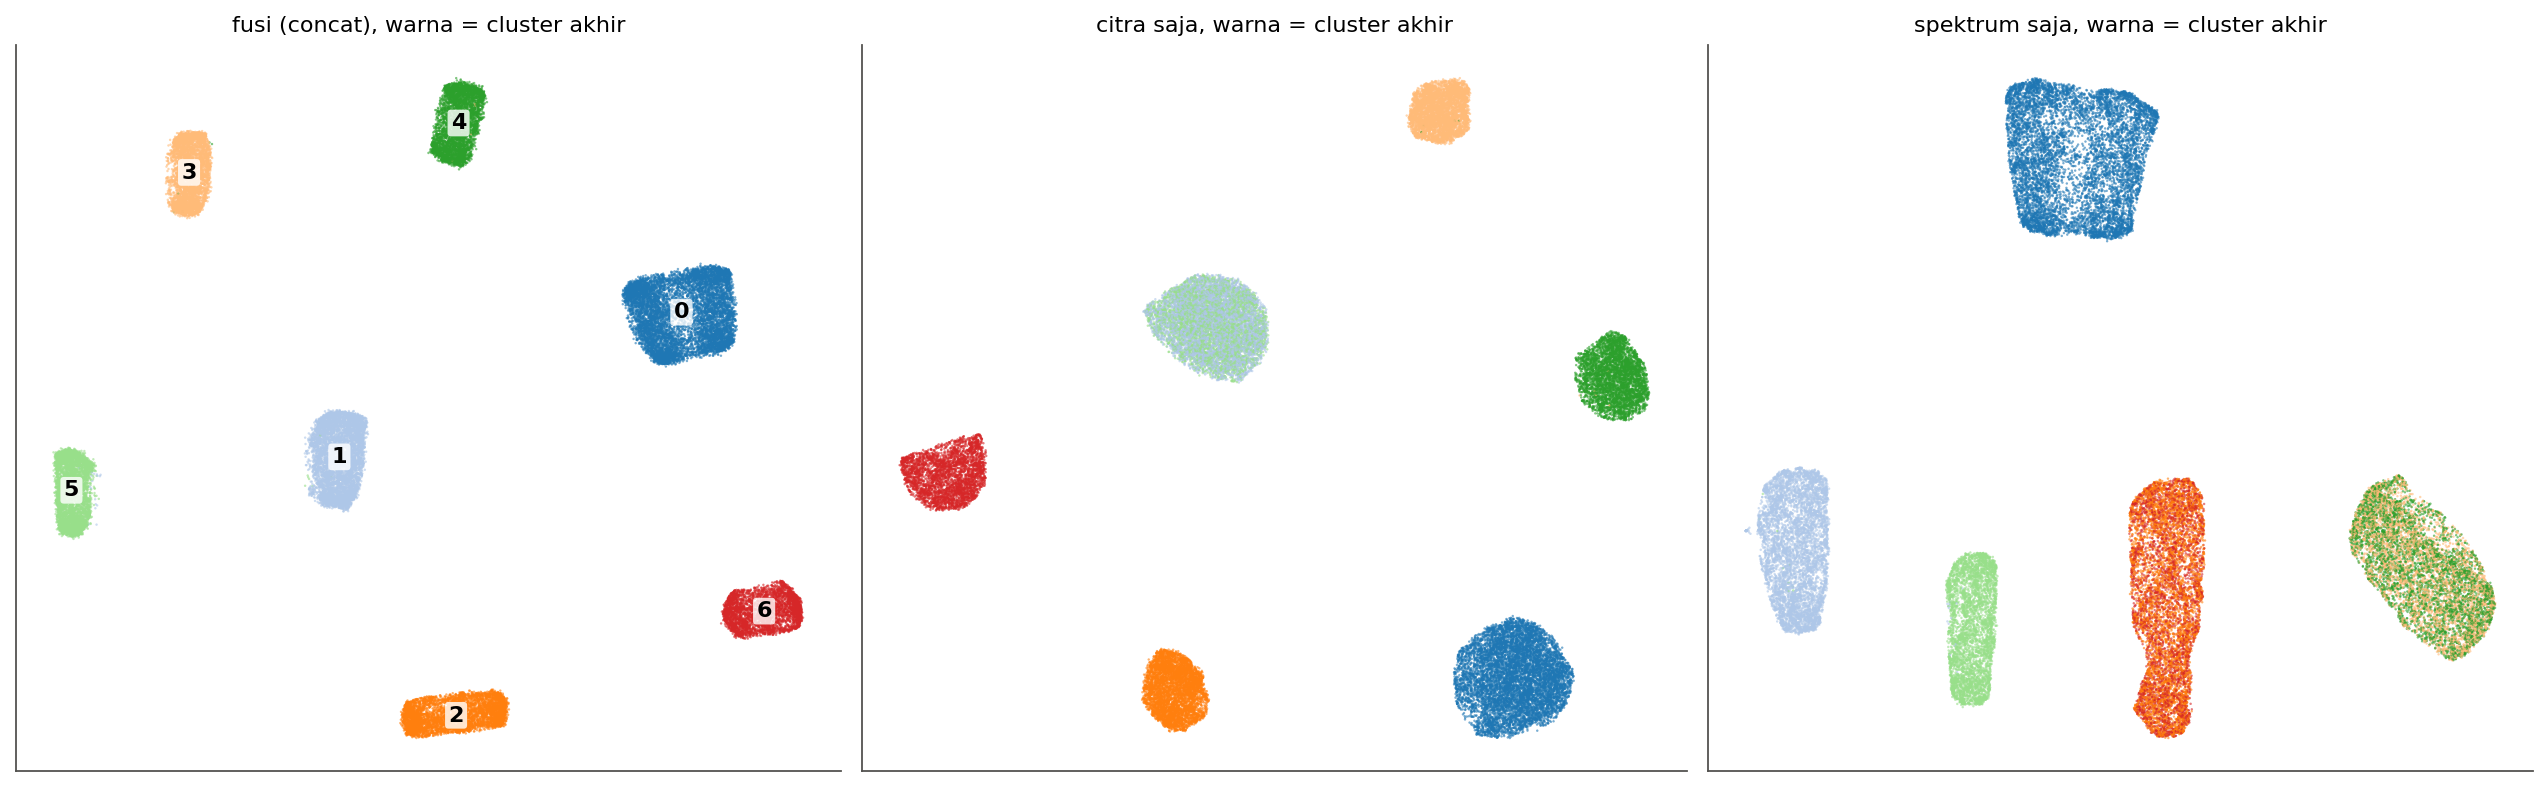
\includegraphics[width=\linewidth]{t3_umap_clusters}
  \caption{UMAP projections~\cite{mcinnes2018umap} coloured by final cluster ID (0--6). Left: fused
  \texttt{concat} embedding cleanly separates all 7 islands. Middle: image-only merges clusters 1
  and 5. Right: spectrum-only merges clusters 3 and 4 (as well as 2 and 6).}
  \label{fig:t3-umap}
\end{figure}

\subsection{Number of clusters and clustering methods}
\label{sec:t3-cluster}

\paragraph{Choosing $K = 7$ over $K = 5$.} We scanned $K = 2 \dots 16$ across six criteria
(Fig.~\ref{fig:t3-k}): five criteria (silhouette 0.320, Davies--Bouldin 1.275,
Calinski--Harabasz 9{,}463, bootstrap ARI stability 0.957, and cross-modal ARI 0.914) peak at
$K = 5$, while GMM BIC decreases monotonically to $K = 16$. Checking the kNN graph ($k = 15$ and
$k = 30$) explains why: the graph has \textbf{5 connected components} (sizes 10{,}043, 8{,}685,
8{,}637, 4{,}979, 3{,}656), giving four zero Laplacian eigenvalues, \emph{followed by two more
near-zero eigenvalues} ($0.0016$ and $0.0031$ at $k=15$) before a $10\times$ spectral gap to the
seventh ($0.0311$). Those two near-zero eigenvalues correspond to two components that each split
into two single-modality islands ($10{,}043 = 5{,}790 + 4{,}253$ for Clusters 1 vs.\ 5;
$8{,}637 = 4{,}341 + 4{,}296$ for Clusters 3 vs.\ 4) with a graph cut of only 0.1--0.2\%. Because
single-modality differences are real distinct material types, we override $K_{\text{auto}} = 5$ to
\textbf{$K = 7$} (based strictly on internal graph and pairwise evidence, never the hidden
reference).

\begin{figure}[t]
  \centering
  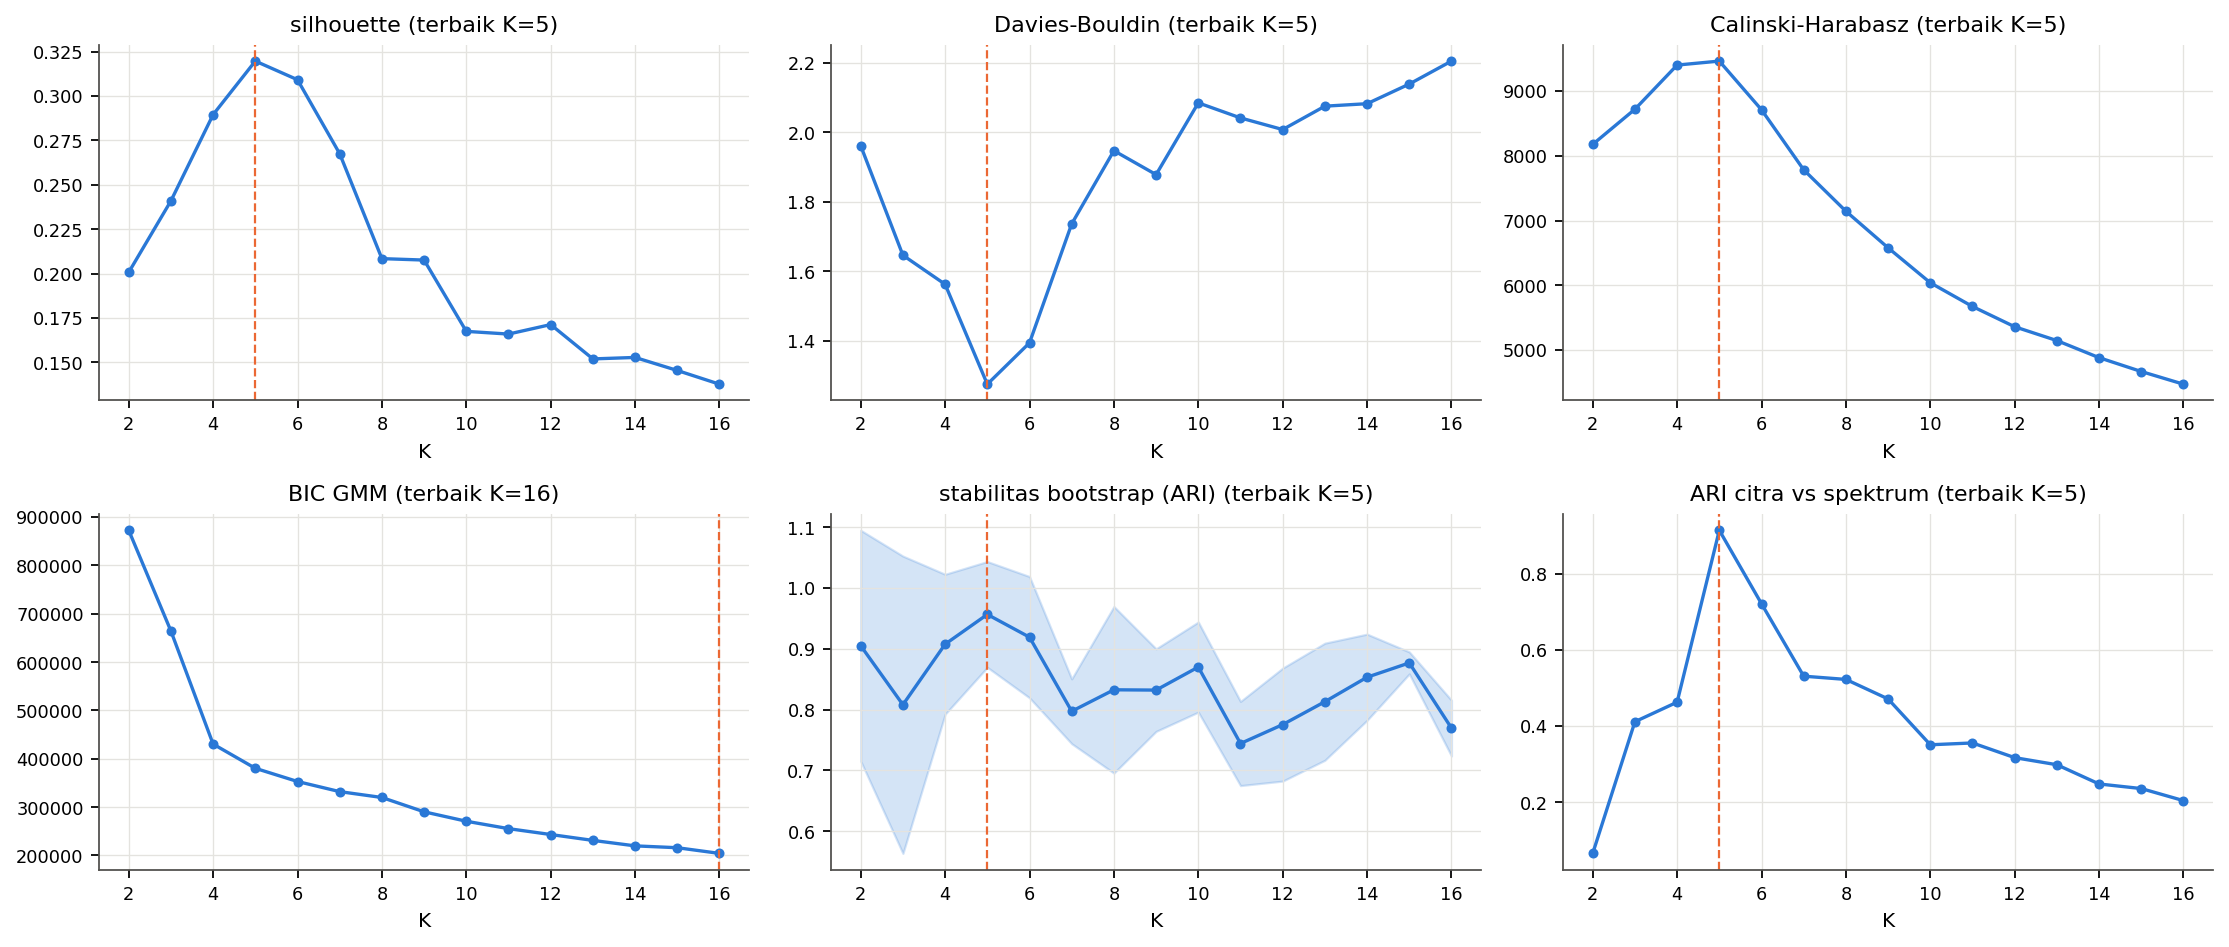
\includegraphics[width=\linewidth]{t3_k_criteria}
  \caption{Cluster-count scan ($K=2 \dots 16$) across six internal criteria on the fused
  \texttt{concat} embedding. Five criteria vote for $K=5$ (the 5 connected components of the kNN
  graph), while Laplacian spectral gap and single-modality island analysis motivate $K=7$.}
  \label{fig:t3-k}
\end{figure}

\paragraph{Comparing five clustering methods (including DEC).} At $K = 7$, we compare KMeans,
full-covariance GMM, Ward/average Agglomerative clustering, kNN graph partitioning, and Deep
Embedded Clustering (DEC~\cite{xie2016dec}, a 60-epoch autoencoder refined for 60 KL-divergence
iterations). Table~\ref{tab:t3-methods} shows that KMeans (kNN cut 1.65\%) and DEC (silhouette
0.220, DB 1.994, kNN cut 2.24\%) cut across dense islands instead of following the thin bridges
between single-modality pairs. In contrast, \textbf{Agglomerative} (kNN cut 0.19\%), GMM (0.12\%),
and Graph partitioning (0.12\%) all recover the exact 7 islands cleanly. We select
\textbf{Agglomerative} on \texttt{concat} for \texttt{cluster.csv} (cluster sizes 3{,}656 to
8{,}685).

\begin{table}[t]
  \centering
  \caption{Clustering methods compared at $K = 7$ on the 64-d fused \texttt{concat} embedding.
  \texttt{kNN cut} is the share of kNN edges crossing between clusters (lower = respects dense
  islands).}
  \label{tab:t3-methods}
  \small
  \begin{tabular}{lrrrrrr}
    \toprule
    Method & Sil.\ fused & Sil.\ img & Sil.\ spec & DB & kNN cut & Seed ARI \\
    \midrule
    KMeans                 & 0.268 & 0.245 & 0.156 & 1.736 & 0.0165 & 0.930 \\
    GMM                    & 0.246 & 0.228 & 0.125 & 1.725 & 0.0012 & 0.784 \\
    \textbf{Agglomerative} & 0.246 & 0.228 & 0.125 & 1.728 & \textbf{0.0019} & --    \\
    Graph (kNN)            & 0.246 & 0.228 & 0.125 & 1.725 & 0.0012 & --    \\
    DEC~\cite{xie2016dec}  & 0.220 & 0.159 & 0.188 & 1.994 & 0.0224 & 0.723 \\
    \bottomrule
  \end{tabular}
\end{table}

\subsection{Visualization, hard-to-separate clusters, and microscope invariance}
\label{sec:t3-analysis}

Both UMAP (Fig.~\ref{fig:t3-umap}) and t-SNE~\cite{vandermaaten2008tsne} (Appendix
Fig.~\ref{fig:t3-tsne}) show seven compact islands with 99.5--100.0\% same-cluster kNN purity per
cluster. Coloring the UMAP by microscope and raw image brightness (Fig.~\ref{fig:t3-mic}) confirms
uniform mixing inside every cluster: M2 share sits within 39.2--40.7\% across all seven clusters
(dataset average 39.9\%; Cram\'er's $V = 0.0096$), verifying that clusters reflect material types
rather than microscope artifacts.

As shown in Fig.~\ref{fig:t3-pairs}, the only cluster pairs with any nonzero neighborhood overlap
are the two single-modality pairs: \textbf{Clusters 1 vs.\ 5} (overlap 0.45\%, $d'_{\text{img}} =
0.06$, $d'_{\text{spec}} = 6.77$) and \textbf{Clusters 3 vs.\ 4} (overlap 0.25\%, $d'_{\text{img}}
= 6.64$, $d'_{\text{spec}} = 0.06$). Every other pair has 0.00\% overlap ($d' \ge 8.8$ in at least
one modality). This explains why those two pairs have lower per-cluster silhouettes (0.116--0.158
for 1/5 and 0.224--0.232 for 3/4, versus 0.301--0.352 for 0/2/6): they share half of their
64-dimensional representation. Note transparently that overriding $K_{\text{auto}}=5 \to 7$ and
choosing Agglomerative by low \texttt{kNN cut} were guided by inspecting the internal graph and
pairwise structure after training.

\begin{figure}[t]
  \centering
  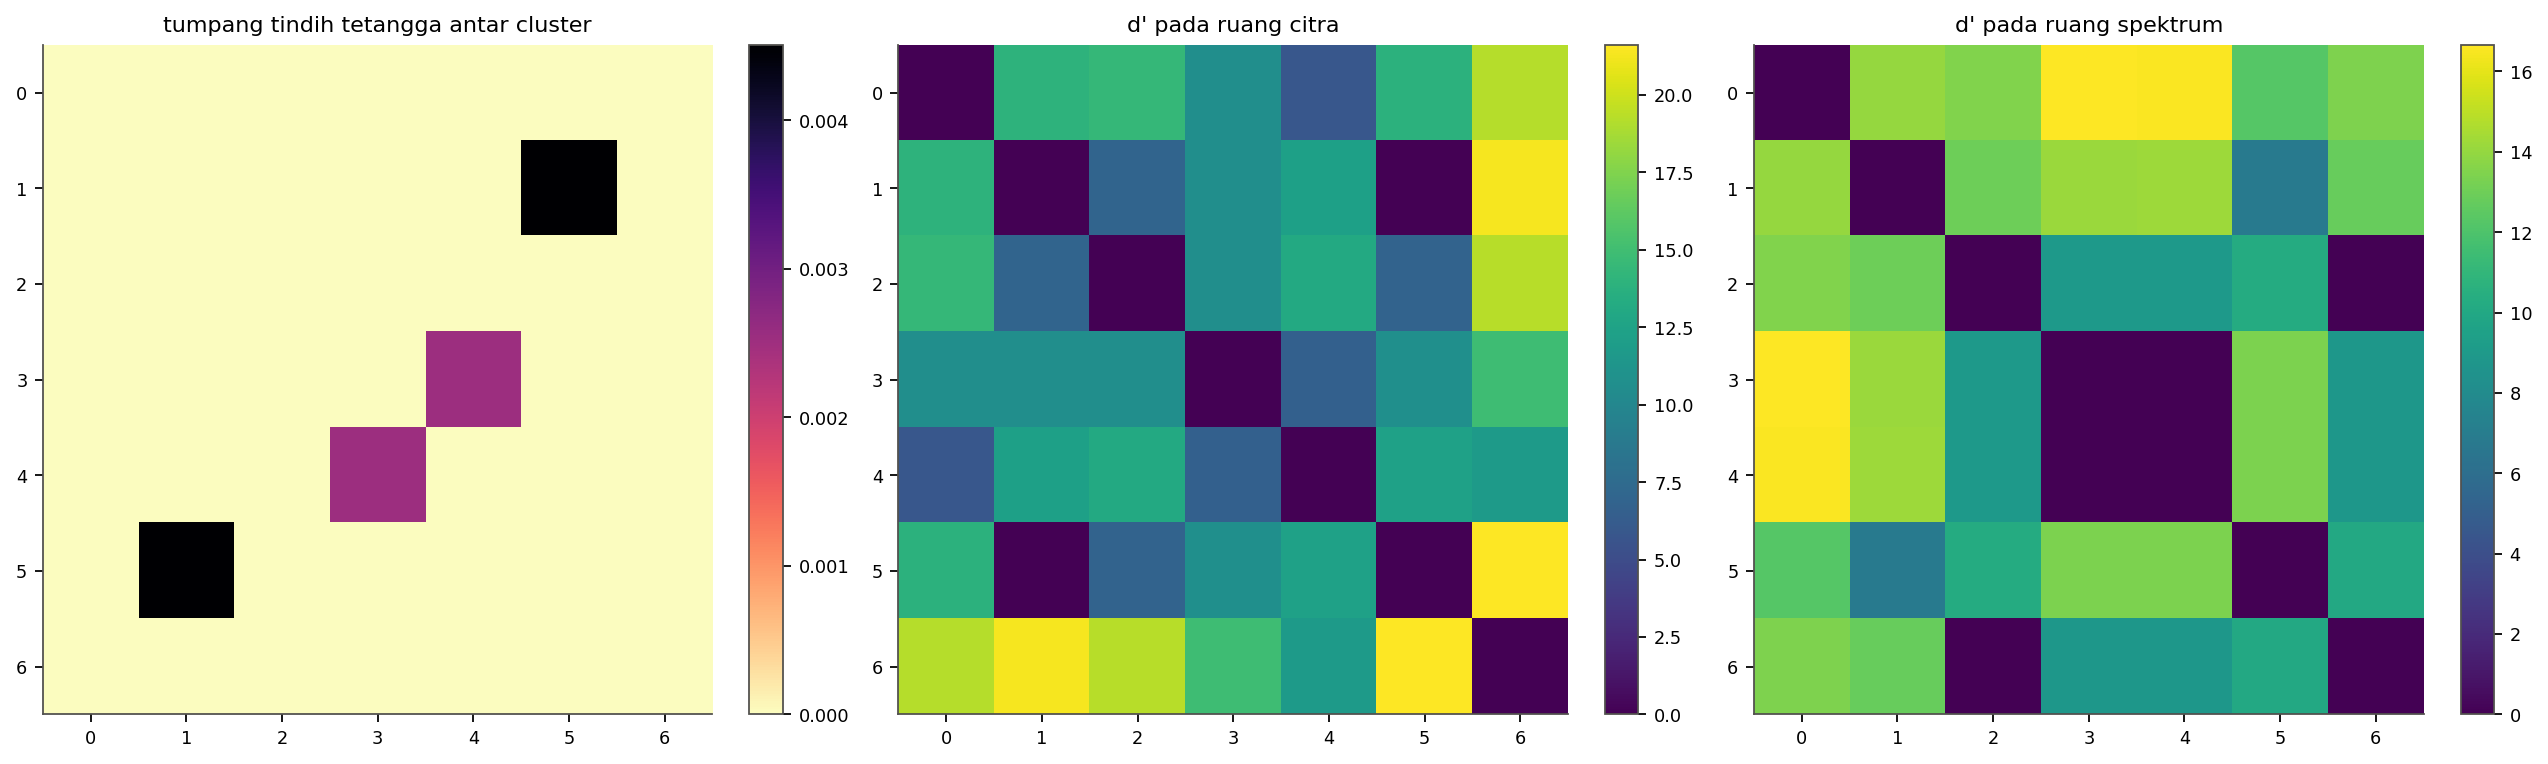
\includegraphics[width=\linewidth]{t3_pair_matrices}
  \caption{Pairwise cluster diagnostics at $K = 7$. Left: kNN boundary overlap (only pairs 1--5
  and 3--4 are nonzero, $\le 0.45\%$). Middle and right: $d'$ separation in image space vs.\
  spectrum space, confirming why single-modality clustering misses one of the two pairs.}
  \label{fig:t3-pairs}
\end{figure}

\begin{figure}[t]
  \centering
  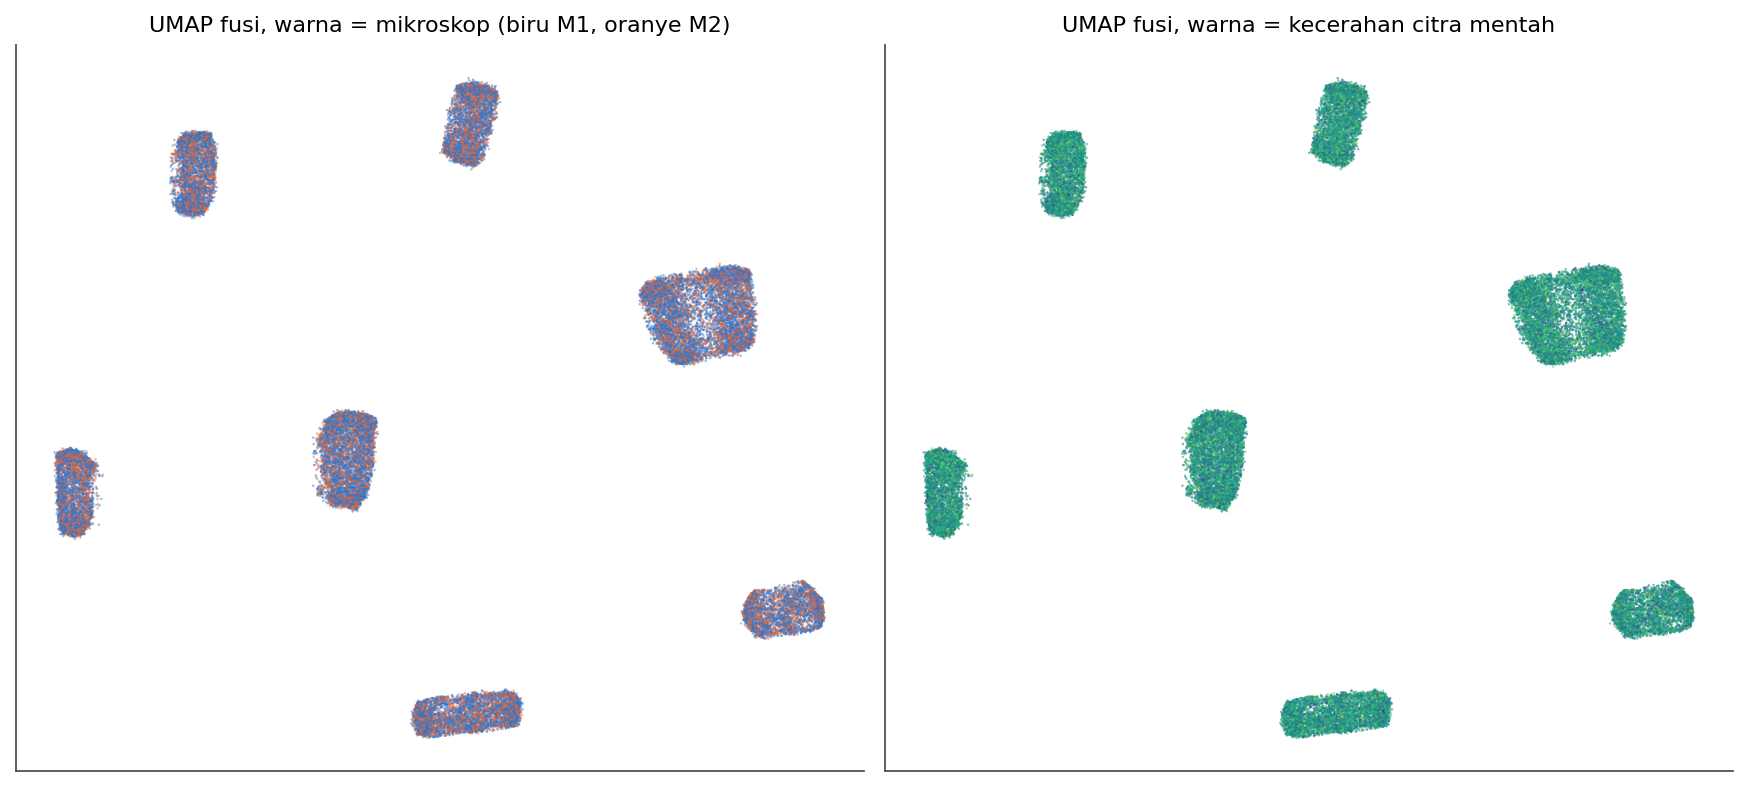
\includegraphics[width=\linewidth]{t3_umap_microscope}
  \caption{Microscope and brightness invariance check on the fused UMAP. Left: M1 (blue) and M2
  (orange) mix uniformly inside every island (Cram\'er's $V = 0.0096$). Right: raw image brightness
  shows no cluster-level bias.}
  \label{fig:t3-mic}
\end{figure}


\bibliographystyle{plain}
\bibliography{refs}

\clearpage  % appendix starts on a new page, so the 18-page limit is easy to check
\appendix
\section{Appendix}
% Appendices (not counted in the 18-page limit).
\input{sections/lampiran_task2}
\clearpage
\subsection{Task 3: supporting material}
\label{app:t3}
% Numbers: kode/results/task3/results.json (python run_all.py --task 3).

\begin{figure}[!htbp]
  \centering
  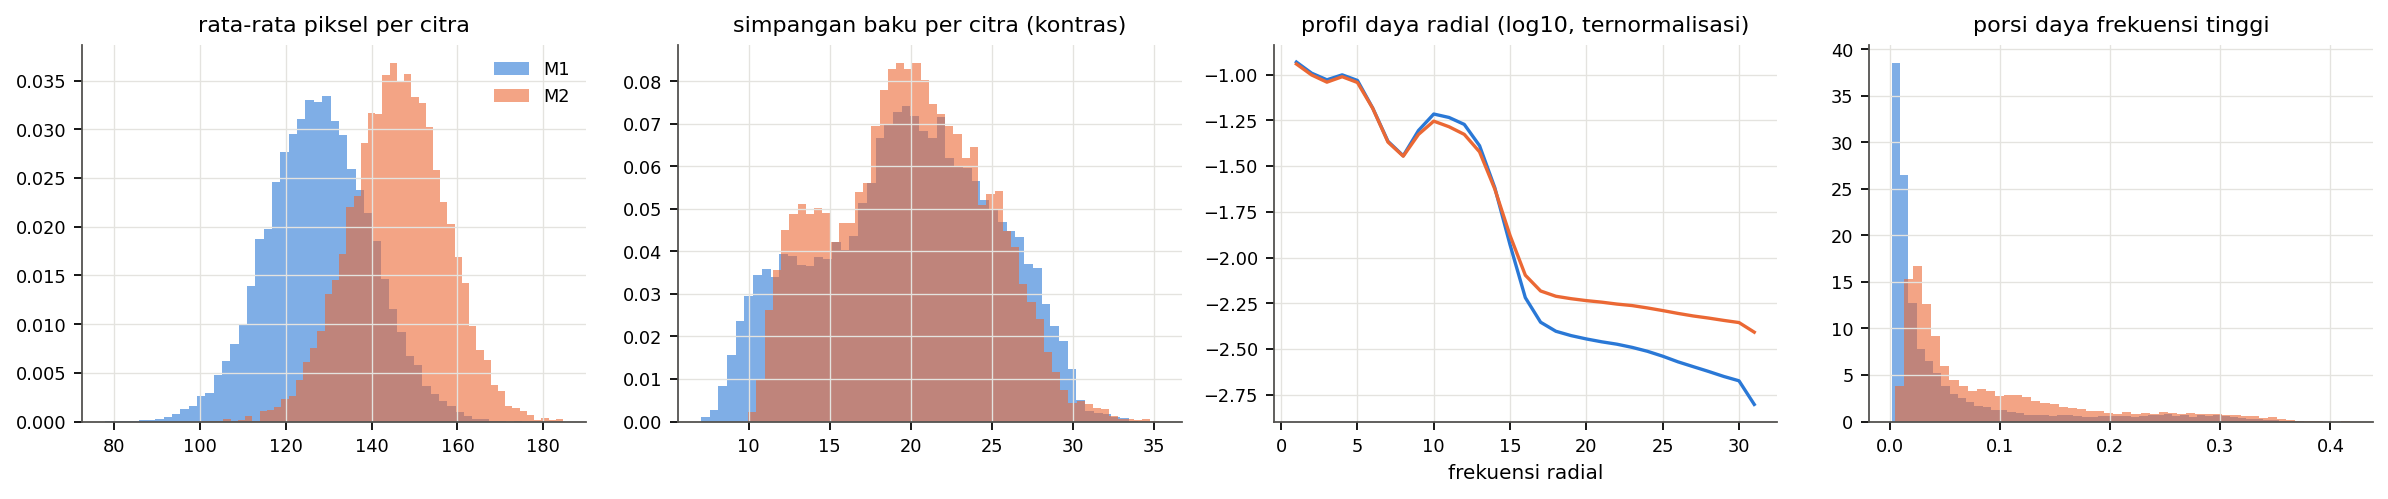
\includegraphics[width=\linewidth]{t3_eda_microscope}
  \caption{Image intensity and frequency-energy distributions across microscopes M1 and M2.}
  \label{fig:t3-eda-mic}
\end{figure}

\begin{figure}[!htbp]
  \centering
  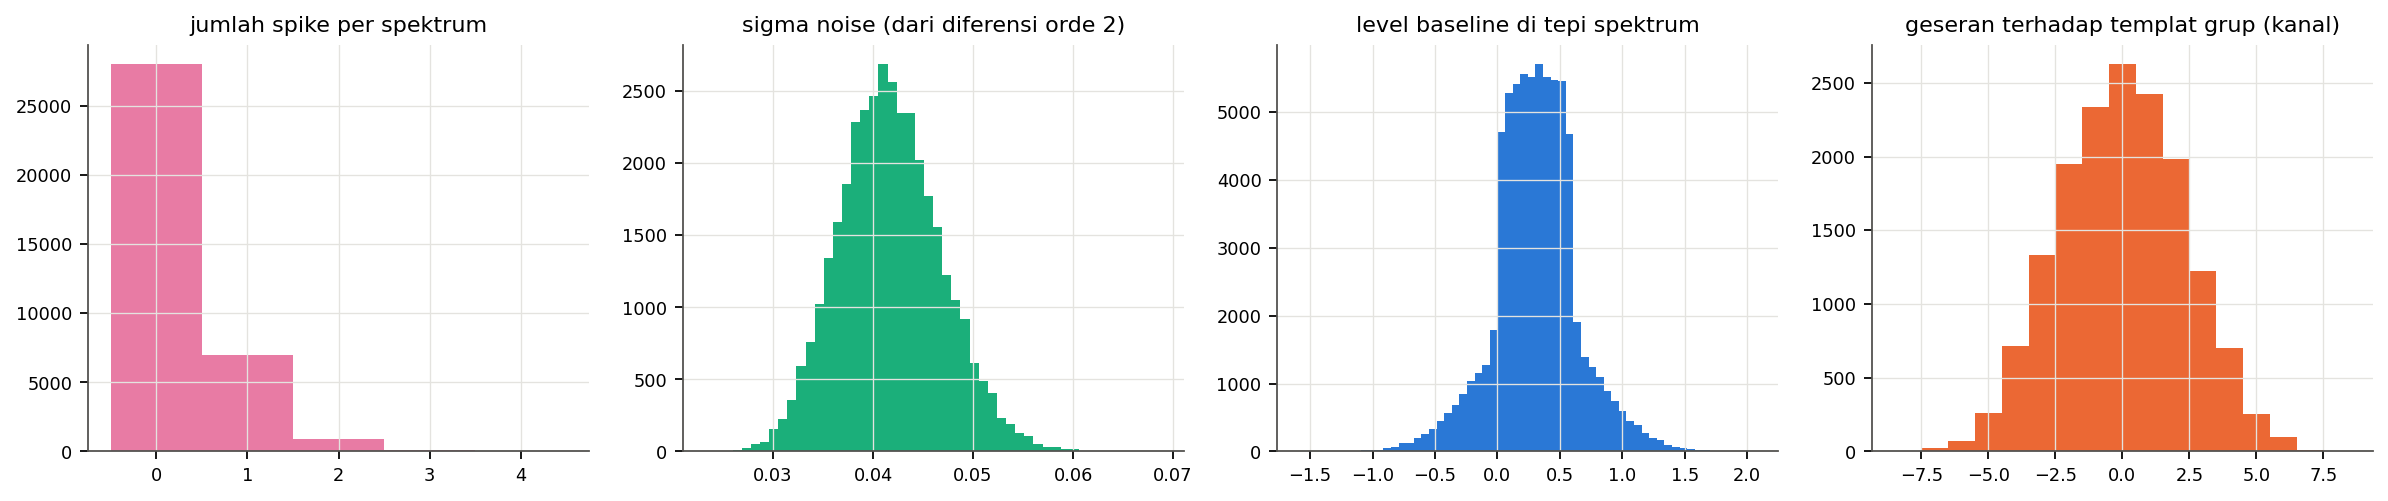
\includegraphics[width=\linewidth]{t3_eda_spectrum_distortions}
  \caption{Spectrum distortions: spikes (22.2\% of samples), baseline offset/tilt, and wavelength shift.}
  \label{fig:t3-eda-spec}
\end{figure}

\begin{figure}[!htbp]
  \centering
  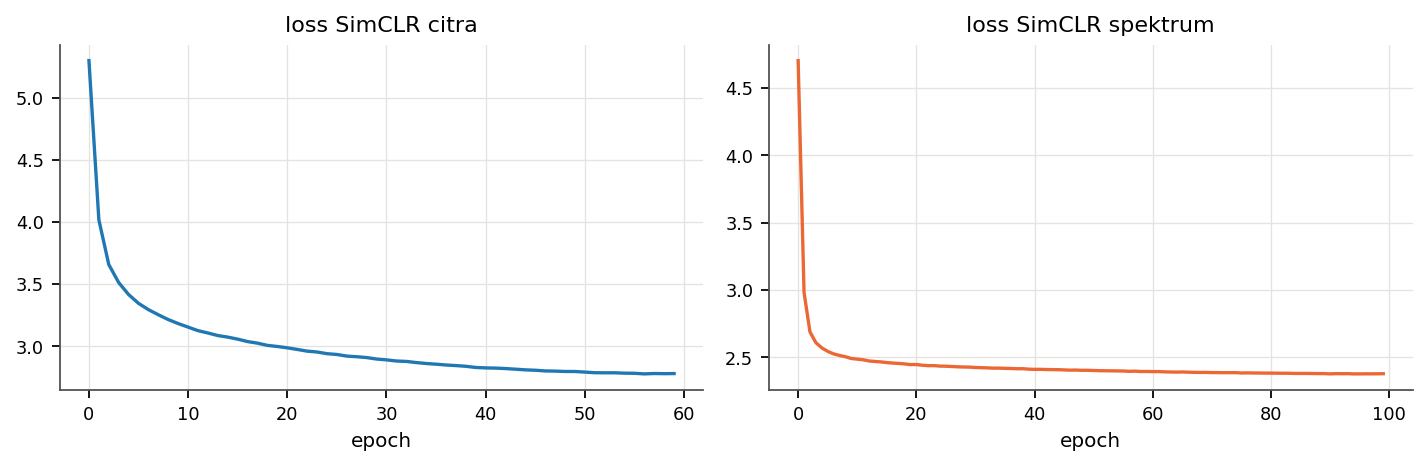
\includegraphics[width=\linewidth]{t3_simclr_loss}
  \caption{SimCLR NT-Xent training loss curves for the image (60 epochs) and spectrum (100 epochs) encoders.}
  \label{fig:t3-loss}
\end{figure}

\begin{figure}[!htbp]
  \centering
  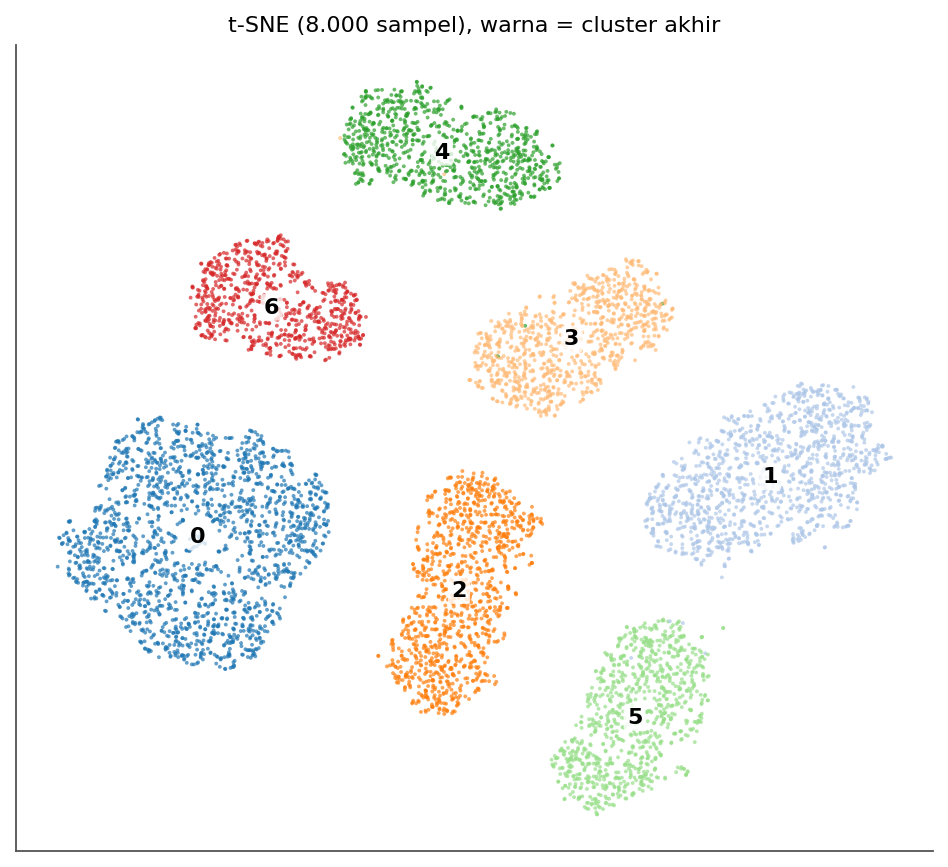
\includegraphics[width=\linewidth]{t3_tsne_clusters}
  \caption{t-SNE~\cite{vandermaaten2008tsne} projection of the fused \texttt{concat} embedding coloured by final cluster ID (0--6).}
  \label{fig:t3-tsne}
\end{figure}

\begin{figure}[!htbp]
  \centering
  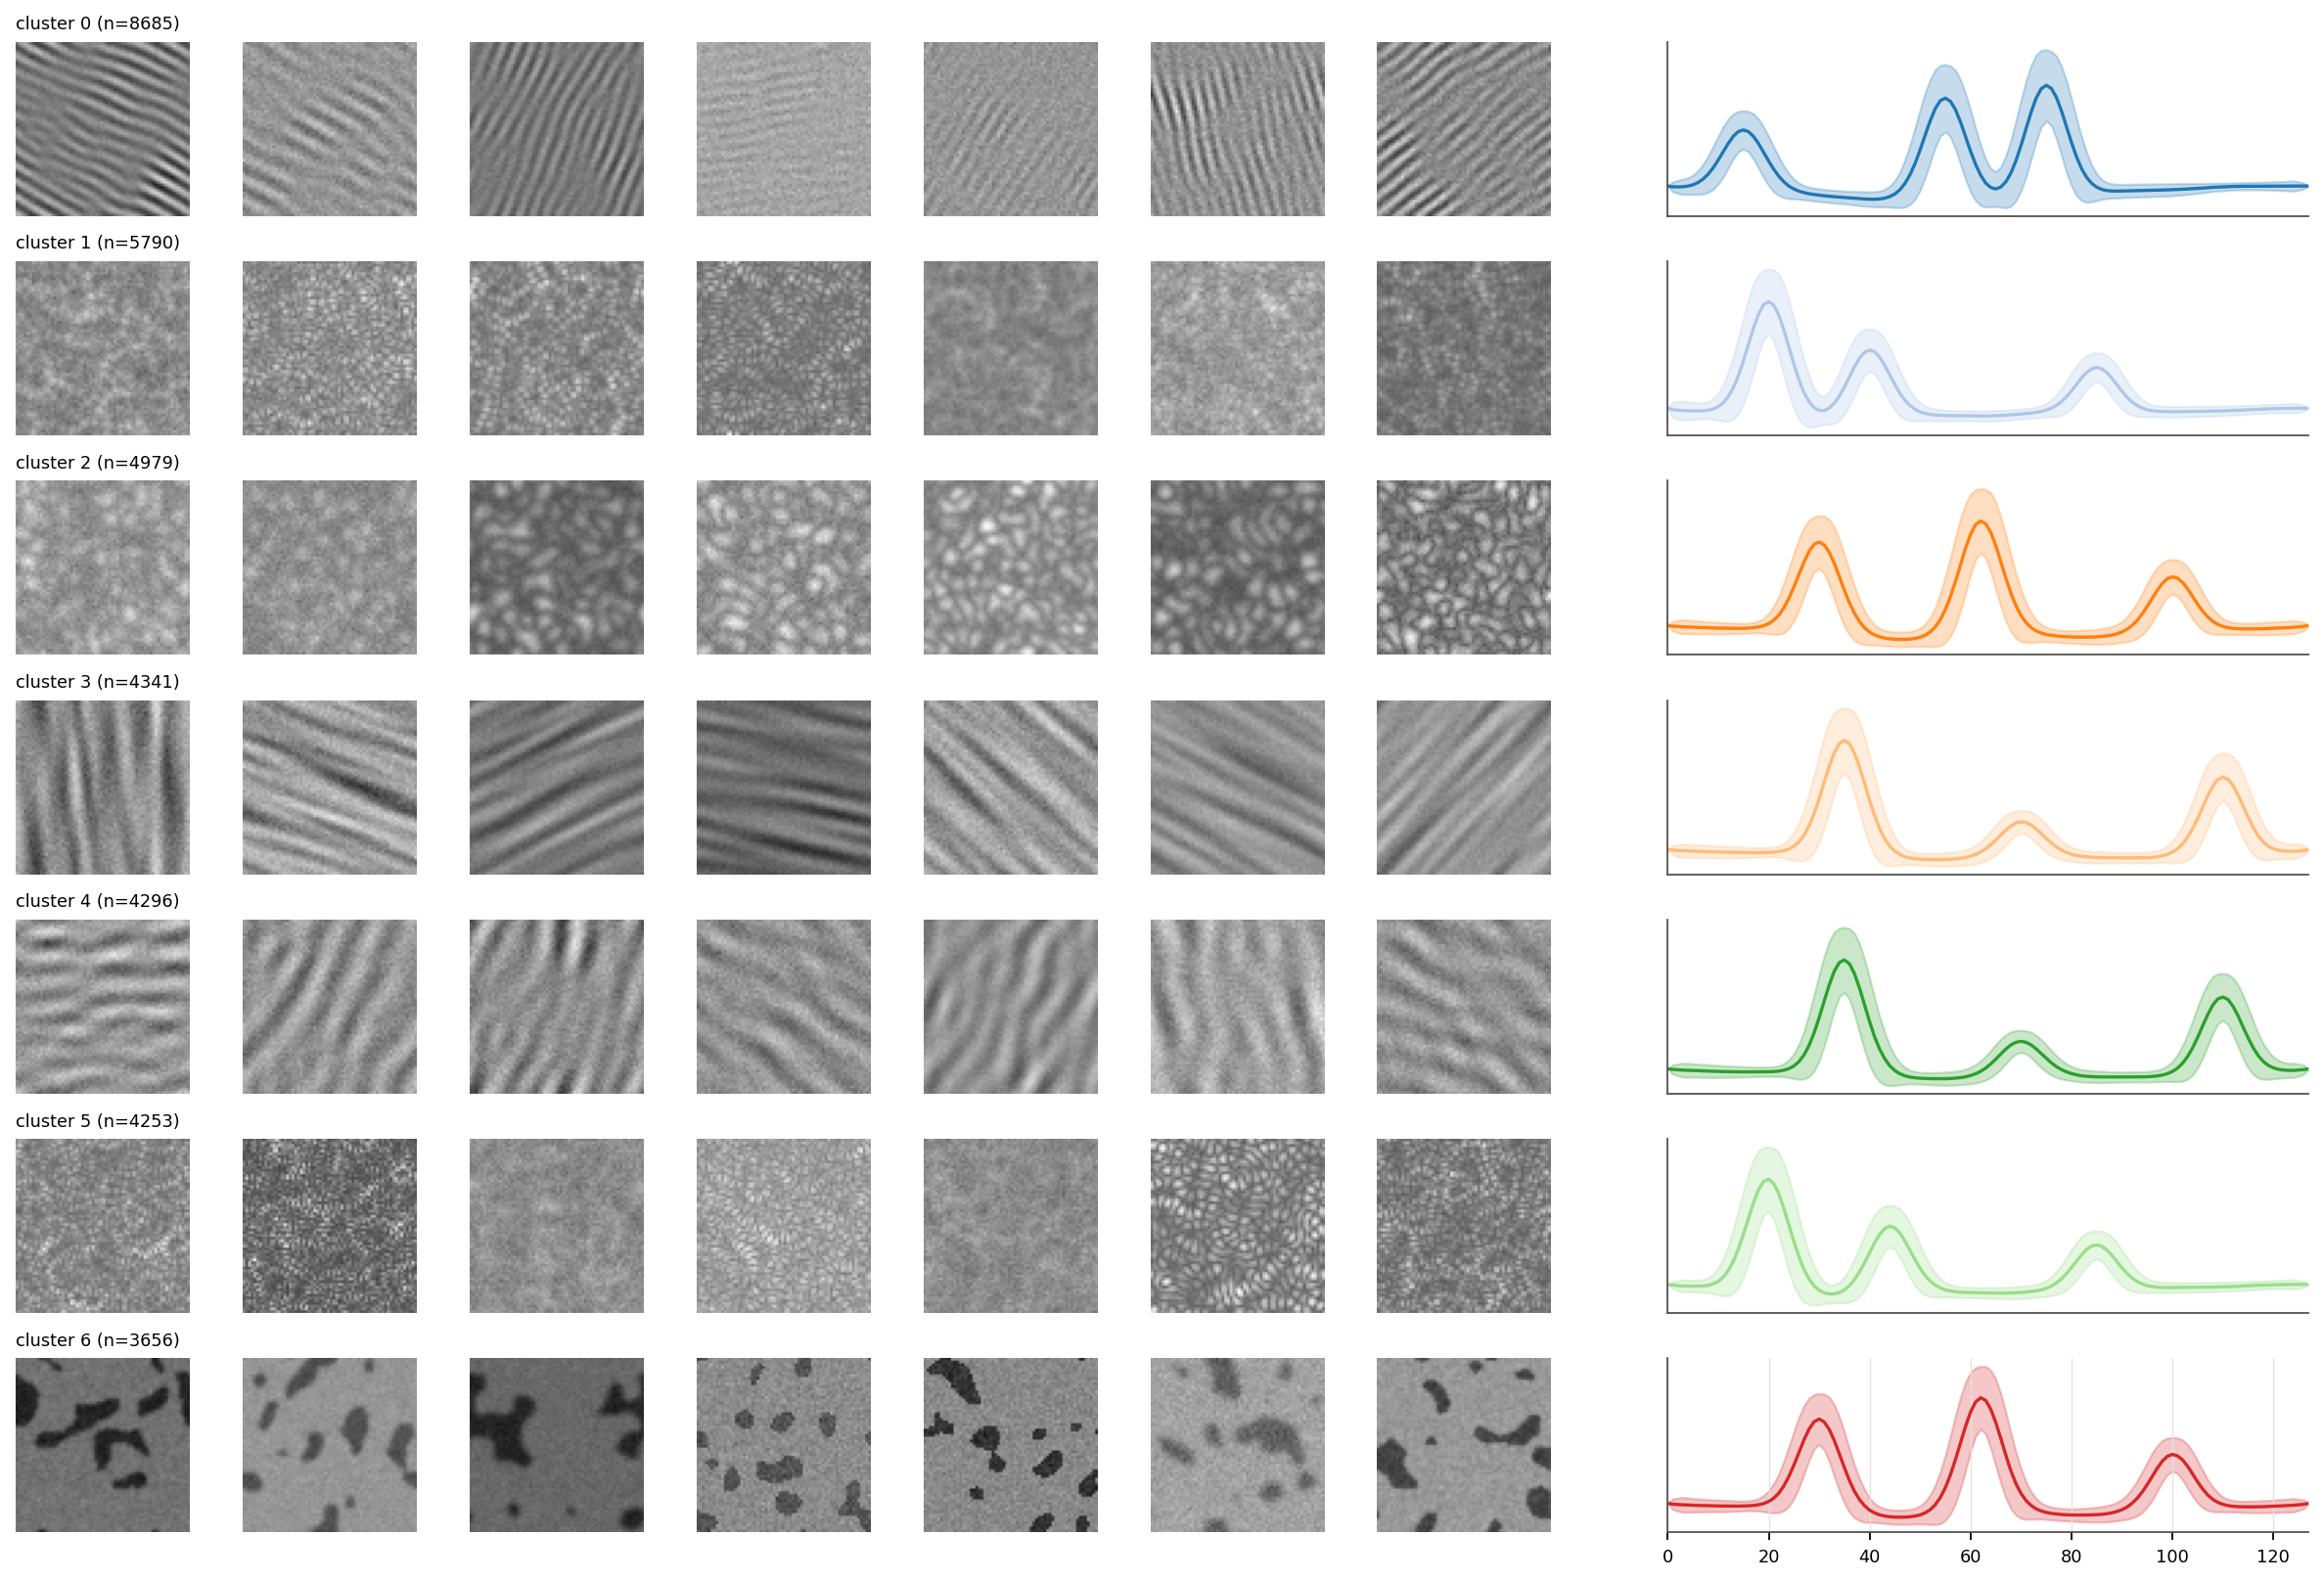
\includegraphics[width=\linewidth]{t3_cluster_profiles}
  \caption{Representative microstructure images and mean preprocessed spectra for each of the 7 clusters.}
  \label{fig:t3-profiles}
\end{figure}



\end{document}
